\documentclass[9pt,twocolumn,twoside]{optica}
\setboolean{shortarticle}{false}
\setboolean{minireview}{false}

\title{Legacy \LaTeX\ template for preparing an article for submission to \emph{Optica}}

\author[1,2,3]{Author One}
\author[2,*]{Author Two}
\author[1]{Author Three}

\affil[1]{Publications Department, The Optical Society, 2010 Massachusetts Avenue NW, Washington DC, 20036, USA}
\affil[2]{School of Science, University of Technology, 2000 J St. NW, Washington DC, 20036, USA}
\affil[3]{School of Optics, University of Technology, 2000 J St. NW, Washington DC, 20036, USA}

\affil[*]{Corresponding author: email@my-email.com}

% To be edited by editor
% \dates{Compiled \today}

%\ociscodes{(140.3490) Lasers, distributed feedback; (060.2420) Fibers, polarization-maintaining; (060.3735) Fiber Bragg gratings.}

% To be edited by editor
% \doi{\url{http://dx.doi.org/10.1364/optica.XX.XXXXXX}}

\begin{abstract}
This legacy \LaTeX\ template can be used to prepare a research article or a short article for submission to \emph{Optica}. Select \texttt{$\setminus$setboolean\{shortarticle\}\{false\}} for a research article or \texttt{$\setminus$setboolean\{shortarticle\}\{true\}} for a letter or memorandum. Select \texttt{$\setminus$setboolean\{minireview\}\{true\}} to output a header identifying the paper as a Mini-Review. Authors may use this legacy template for a precise length estimate for \emph{Optica} letters and memoranda. Please note that OSA is no longer using OCIS codes.
\end{abstract}

\setboolean{displaycopyright}{true}

\begin{document}

\maketitle

\section{Introduction}

This legacy template is designed to assist with creating a two-column research article or letter to submit to \emph{Optica}. See the OSA's \href{http://www.opticsinfobase.org/submit/style/}{Style Guide} and \href{http://www.opticsinfobase.org/submit/templates/}{Manuscript Templates} pages for more details.

If you have a question while using this template on \href{https://www.overleaf.com}{Overleaf}, please use the help menu (``?'') on the top bar to search for help or ask us a question using the option in the lower right of the editor.

\section{Examples of Article Components}
\label{sec:examples}

The sections below show examples of different article components. Sections should generally follow the conventional order: Introduction, Method, Results, Discussion, and Conclusion.  Please do not include Methods in a separate section at the end.

\section{Figures and Tables}

It is not necessary to place figures and tables at the back of the manuscript. Figures and tables should be sized as they are to appear in the final article. Do not include a separate list of figure captions and table titles.

Figures and Tables should be labeled and referenced in the standard way using the \verb|\label{}| and \verb|\ref{}| commands.

\subsection{Sample Figure}

Figure \ref{fig:false-color} shows an example figure.

\begin{figure}[htbp]
\centering
\fbox{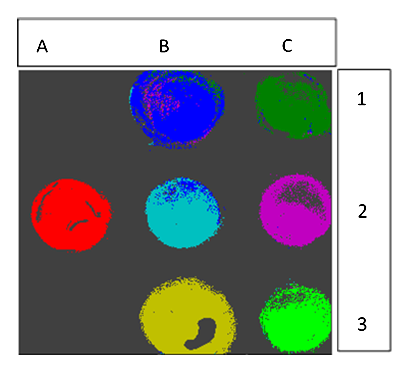
\includegraphics[width=\linewidth]{sample}}
\caption{False-color image, where each pixel is assigned to one of seven reference spectra.}
\label{fig:false-color}
\end{figure}

\subsection{Sample Table}

Table \ref{tab:shape-functions} shows an example table.

\begin{table}[htbp]
\centering
\caption{\bf Shape Functions for Quadratic Line Elements}
\begin{tabular}{ccc}
\hline
local node & $\{N\}_m$ & $\{\Phi_i\}_m$ $(i=x,y,z)$ \\
\hline
$m = 1$ & $L_1(2L_1-1)$ & $\Phi_{i1}$ \\
$m = 2$ & $L_2(2L_2-1)$ & $\Phi_{i2}$ \\
$m = 3$ & $L_3=4L_1L_2$ & $\Phi_{i3}$ \\
\hline
\end{tabular}
  \label{tab:shape-functions}
\end{table}

\section{Sample Equation}

Let $X_1, X_2, \ldots, X_n$ be a sequence of independent and identically distributed random variables with $\text{E}[X_i] = \mu$ and $\text{Var}[X_i] = \sigma^2 < \infty$, and let
\begin{equation}
S_n = \frac{X_1 + X_2 + \cdots + X_n}{n}
      = \frac{1}{n}\sum_{i}^{n} X_i
\label{eq:refname1}
\end{equation}
denote their mean. Then as $n$ approaches infinity, the random variables $\sqrt{n}(S_n - \mu)$ converge in distribution to a normal $\mathcal{N}(0, \sigma^2)$.

\section{Sample Algorithm}

Algorithms can be included using the commands as shown in Algorithm \ref{alg:euclid}.

\begin{algorithm}
\caption{Euclid’s algorithm}\label{alg:euclid}
\begin{algorithmic}[1]
\Procedure{Euclid}{$a,b$}\Comment{The g.c.d. of a and b}
\State $r\gets a\bmod b$
\While{$r\not=0$}\Comment{We have the answer if r is 0}
\State $a\gets b$
\State $b\gets r$
\State $r\gets a\bmod b$
\EndWhile\label{euclidendwhile}
\State \textbf{return} $b$\Comment{The gcd is b}
\EndProcedure
\end{algorithmic}
\end{algorithm}

\section*{Funding Information}
National Science Foundation (NSF) (1263236, 0968895, 1102301); The 863 Program (2013AA014402).

\section*{Acknowledgments}

Formal funding declarations should not be included in the acknowledgments but in a Funding Information section as shown above. The acknowledgments may contain information that is not related to funding:

The authors thank H. Haase, C. Wiede, and J. Gabler for technical support.

\section*{Disclosures}

Disclosures should be listed in a separate section at the end of the manuscript. List the Disclosures codes identified on OSA's \href{http://www.osapublishing.org/submit/review/conflicts-interest-policy.cfm}{Conflict of Interest policy page}. If there are no disclosures, then list ``The authors declare no conflicts of interest.''

Here are examples of disclosures:

\medskip

\noindent\textbf{Disclosures.} ABC: 123 Corporation (I,E,P), DEF: 456 Corporation (R,S). GHI: 789 Corporation (C).

\medskip

\noindent\textbf{Disclosures.} The authors declare no conflicts of interest.

\section*{Supplemental Documents}
\emph{Optica} authors may include supplemental documents with the primary manuscript. For details, see \href{http://www.opticsinfobase.org/submit/style/supplementary-materials-optica.cfm}{Supplementary Materials in Optica}. To reference the supplementary document, the statement ``See Supplement 1 for supporting content.'' should appear at the bottom of the manuscript (above the references).

%\bigskip \noindent See \href{link}{Supplement 1} for supporting content.

\section*{References}

For references, you may add citations manually or use BibTeX. E.g. \cite{Zhang:14}.

Letter submissions to \emph{Optica} require two sets of references: an abbreviated reference style for publication and a full reference list to aid the editor and reviewers. Citations to journal articles in the abbreviated list should omit the article title and final page number; this abbreviated reference style is produced automatically when the \texttt{$\setminus$setboolean\{shortarticle\}\{true\}} option is selected in the template, if you are using a .bib file for your references.
 
The full reference list meant to aid the editor and reviewers must be included as well on an informational page that will not count against page length; again this will be produced automatically if you are using a .bib file and have the \texttt{$\setminus$setboolean\{shortarticle\}\{true\}} option selected.


% Bibliography
\bibliography{sample}

% Full bibliography will be added automatically on a new page for Optics Letters submissions. This command is ignored for journal article submissions.
% Note that this extra page will not count against page length.
\bibliographyfullrefs{sample}

%Manual citation list
%\begin{thebibliography}{1}
%\bibitem{Zhang:14}
%Y.~Zhang, S.~Qiao, L.~Sun, Q.~W. Shi, W.~Huang, %L.~Li, and Z.~Yang,
 % \enquote{Photoinduced active terahertz metamaterials with nanostructured
  %vanadium dioxide film deposited by sol-gel method,} Opt. Express \textbf{22},
  %11070--11078 (2014).
%\end{thebibliography}

\end{document} 